\section{Requirements}

PARK ist eine Software-as-a-Service (SaaS) Anwendung für die Verwaltung von Parkeinrichtungen für Gemeinden, oder Unternehmen.
Die Anwendung stellt eine umfassende Palette an Funktionen bereit, um den Parkbetrieb zu optimieren, 
die User Experience zu verbessern und die Verwaltung der Parkinfrastruktur effizienter zu gestalten.  \\


\textbf{Hauptziele:}

\begin{itemize}
    \item \textbf{Integration in die Parkinfrastruktur:} Die Anwendung wird in die Parkbereichs- und Garageninfrastruktur integriert, um die automatisierte Ein- und Ausfahrt von Fahrzeugen, sowie die Verifizierung von Zahlungen für Park- und Ladevorgänge zu ermöglichen.
    \item \textbf{Verwaltung der Parkinfrastruktur:} Die Parkinfrastruktur wird digital abgebildet und kann flexibel an Veränderungen in der realen Welt angepasst werden. Die Integration mit den Prozessen für Parken und Laden sowie mit der Mängelverwaltung ermöglicht umfangreiche Analysen und einen ganzheitlichen Überblick über die Infrastruktur
    \item \textbf{Globale Bereitstellung:} Die SaaS Anwendung ist für globale Skalierbarkeit ausgelegt und ermöglicht eine automatisierte Bereitstellung für Kunden mit unterschiedlichen Bedürfnissen.
\end{itemize}


Funktional ermöglicht die Anwendung die digitale Abbildung der realen Infrastruktur, um die Belegung, Parkflächen, Ladestationen, Mängel und Benutzer an zentraler Stelle zu verwalten. Umfassende Benutzerverwaltung erlaubt verschiedene Sichten auf die Applikation, sodass alle Stakeholder ihren Bedürfnissen entsprechend Zugang zu unterschiedlichen Funktionen erhalten. Automatisierte Bereitstellung ermöglicht es für Tenants mit unterschiedlichen Bedürfnissen, eine auf sie zugeschnittene Instanz der Anwendung erstellen zu können.


\subsection{System Context}

Das System läuft im Kontext unterschiedlicher interner und externer Komponenten. Interne Komponenten beschreiben dabei Komponenten, die vom Solution Administrator selbst verwaltet werden, über die er/sie also eine gewisse Kontrolle hat. Externe Komponenten sind dann alle diejenigen, über die der Solution Administrator keine Kontrolle hat. 

In Abbildung \ref{fig:context-diagram} ist der Systemkontext und die Interaktion mit der Solution in einem Kontextdiagramm dargestellt.

\begin{figure}[H]
    \centering
    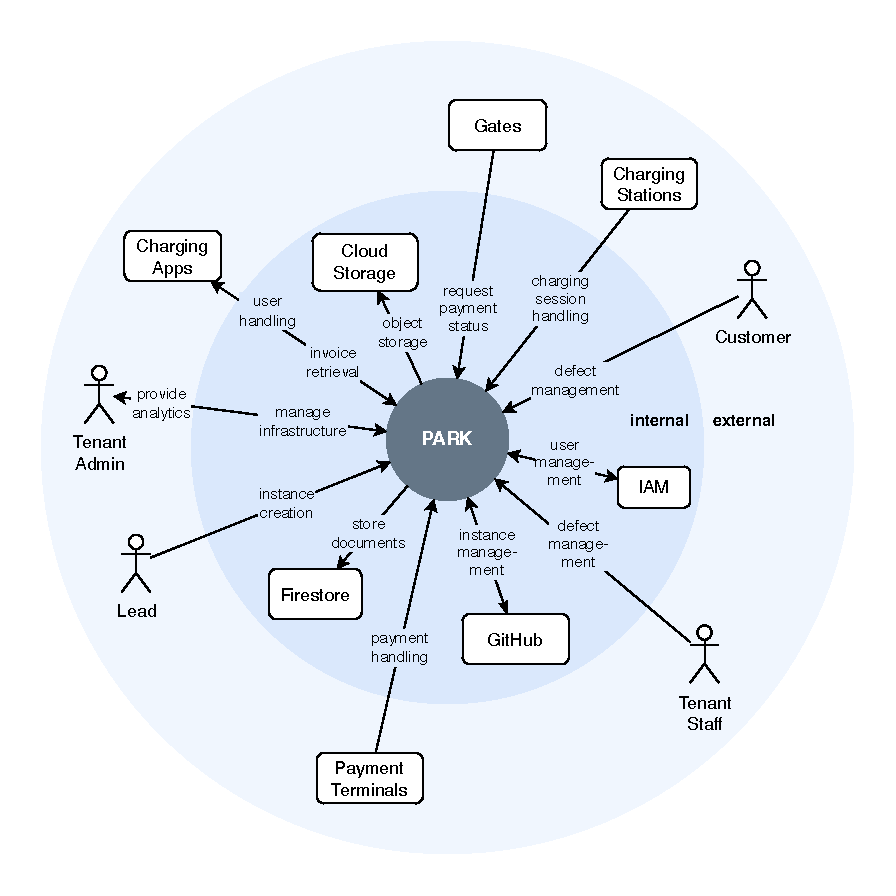
\includegraphics[width=0.9\textwidth]{resources/context-diagram.pdf}
    \caption{Context Diagram}
    \label{fig:context-diagram}
\end{figure}


\subsection{Use Case Overview}
Im folgenden Abschnitt werden die Use Cases der Parking Management Lösung genauer beschrieben. Diese Aktoren existieren in diesem Kontext:

\renewcommand{\arraystretch}{1.5}
{\rowcolors{2}{}{gray!20}
\begin{longtable}{l p{10cm}}
    \caption{Use Case Aktoren}
    \label{tab:use-case-actors} \\
    \textbf{Actor} & \textbf{Beschreibung} \\ [1ex]
    Customer & Der Endkunde, der die Parking Infrastruktur nutzt \\ [0.5ex]
    Tenant Staff & Mitarbeiter (bspw. Financial oder Operations) des Tenants \\ [0.5ex]
    Tenant Administrator & Administrator auf Tenant-Ebene \\ [0.5ex]
    Solution Administrator & Administrator, der die Lösung bereitstellt \\ [0.5ex]
    Lead & Potenzielle Kunden, die eine Instanz der Lösung erstellen möchten \\ 
\end{longtable}}

Zusätzlich zu den Aktoren, die entsprechende Personen darstellen, existieren noch sogenannte System Actors. Damit sind die Systemkomponenten gemeint, sie auch als Aktoren mit anderen Systemkomponenten interagieren. Dies sind beispielsweise externe Komponenten wie die Ladestationen, Schranken, 3rd Party Applikationen des E-Charging Anbieters, aber auch die Microservices der Lösung, die untereinander interagieren.

Das Parking Management bündelt sämtliche Funktionalität für die Abwicklung der Prozesse rund um das Parken und Laden. In Abbildung \ref{fig:park-ma-use-cases} sind die Use Cases des Parking Managements abgebildet.

\begin{figure}[H]
    \centering
    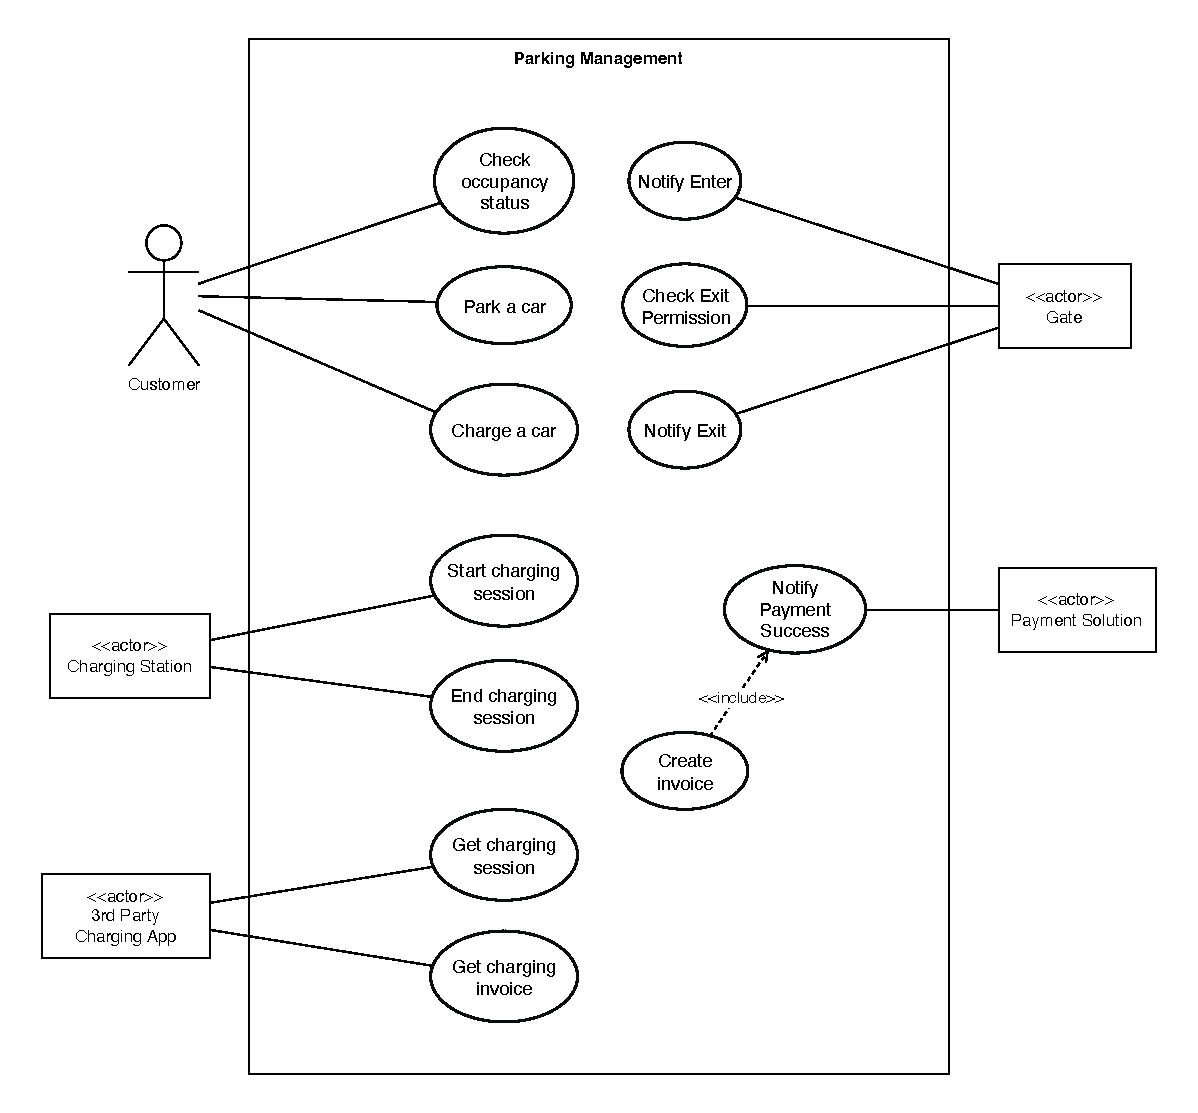
\includegraphics[width=\textwidth]{resources/park-ma-use-cases.pdf}
    \caption{Parking Management Use Cases}
    \label{fig:park-ma-use-cases}
\end{figure}

Das Property Management umfasst alle Funktionen für das Erstellen, Verwalten und Löschen der digitalen Abbildungen der Infrastruktur, sowie das Defect Management.
In Abbildung \ref{fig:prop-ma-use-cases} sind alle Use Cases für des Property Managements dargestellt.

\begin{figure}[H]
    \centering
    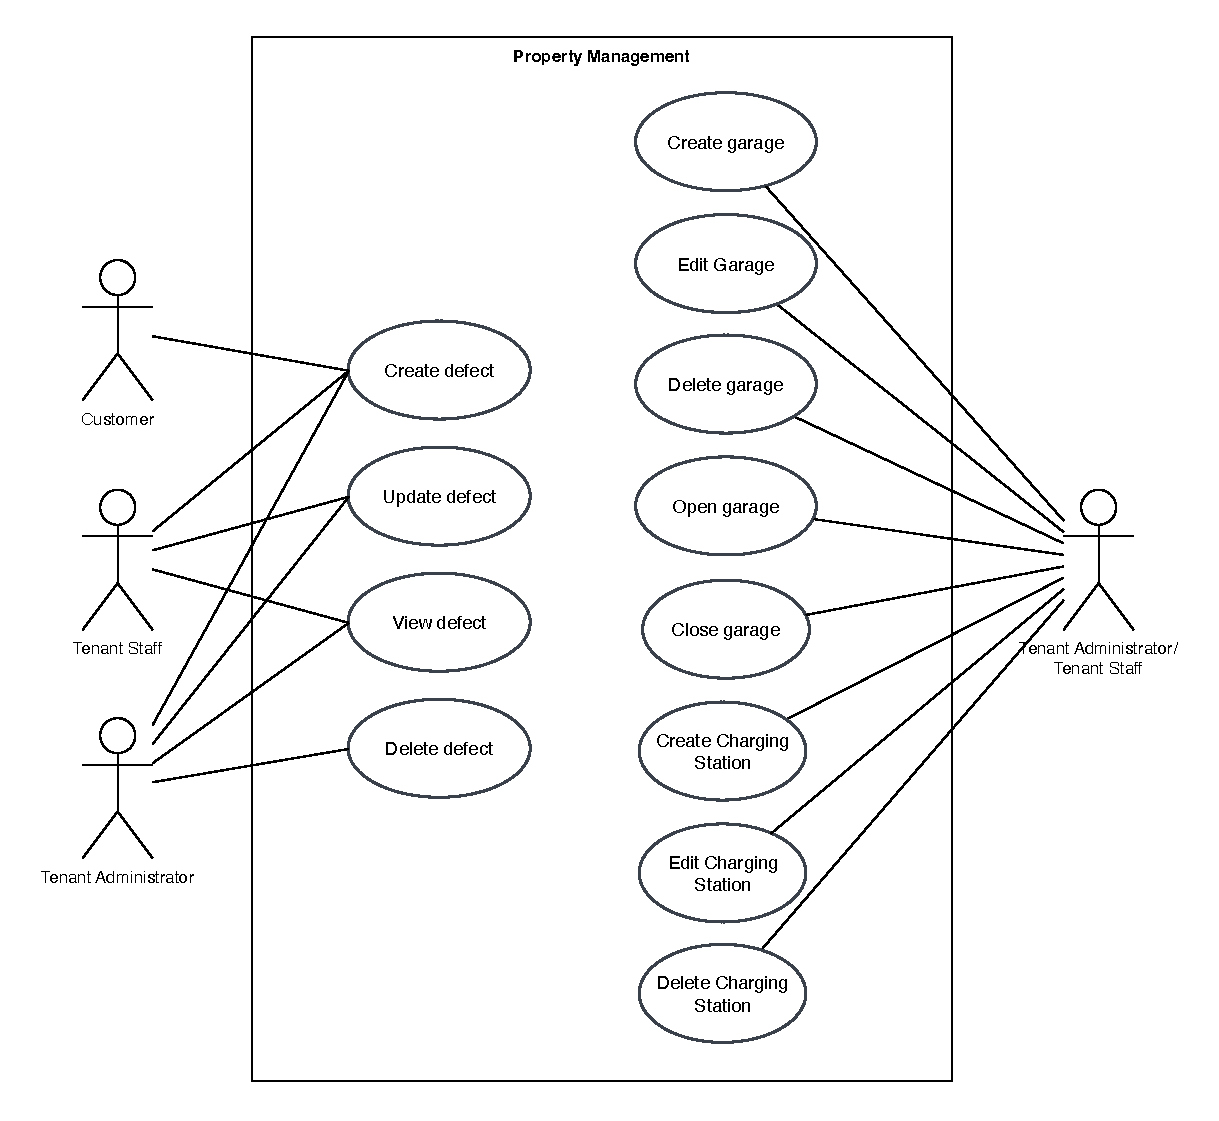
\includegraphics[width=\textwidth]{resources/prop-ma-use-cases.pdf}
    \caption{Property Management Use Cases}
    \label{fig:prop-ma-use-cases}
\end{figure}

Infrastructure Management umfasst die Verwaltung der Infrastruktur auf Anwendungsebene. Dazu gehören beispielweise die Instanz-Erstellung für neue Tenants und die gesamte Funktionalität für das konsolidieren und abrufen von anwendungsweiten Analytics. Abbildung \ref{fig:inf-ma-use-cases} zeigt die Use Cases für das Infrastructure Management.

\begin{figure}[H]
    \centering
    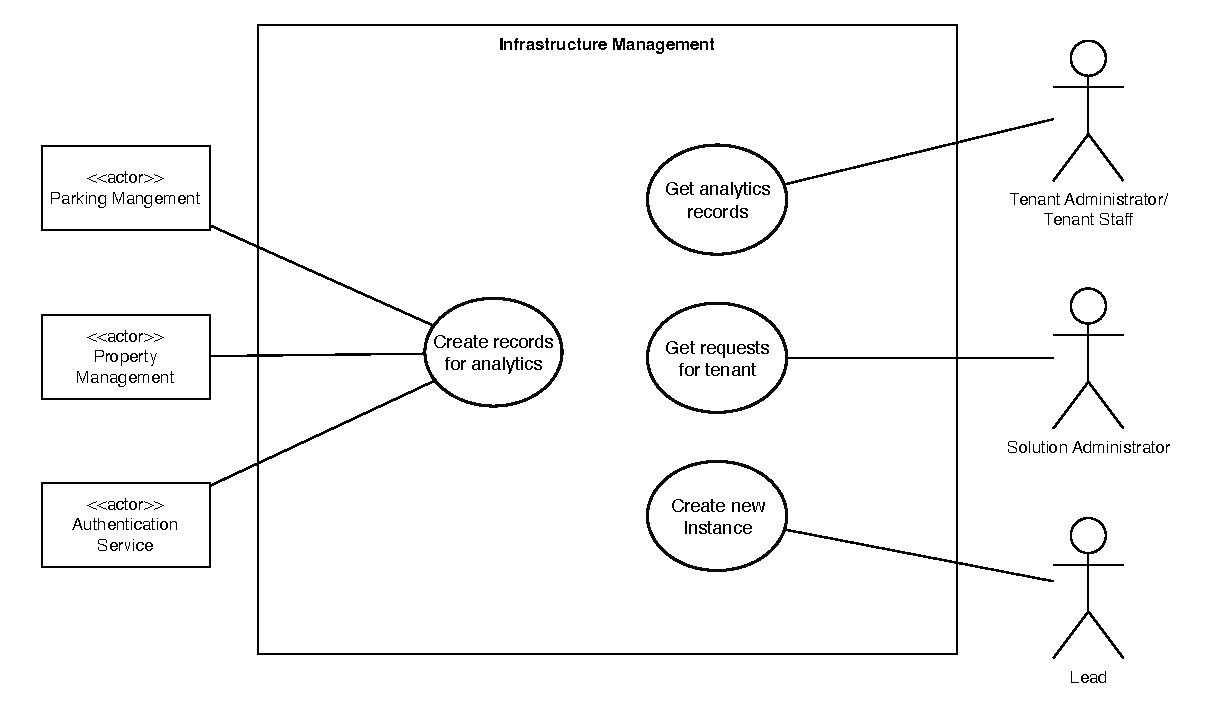
\includegraphics[width=\textwidth]{resources/inf-ma-use-cases.pdf}
    \caption{Infrastructure Management Use Cases}
    \label{fig:inf-ma-use-cases}
\end{figure}

Die Authentication Komponente der Parking Management Solution stellt einige erweiternde Funktionen zur Google Identity Platform bereit. In Abbildung \ref{fig:auth-use-cases} sind die entsprechenden Use Cases dargestellt.


\begin{figure}[H]
    \centering
    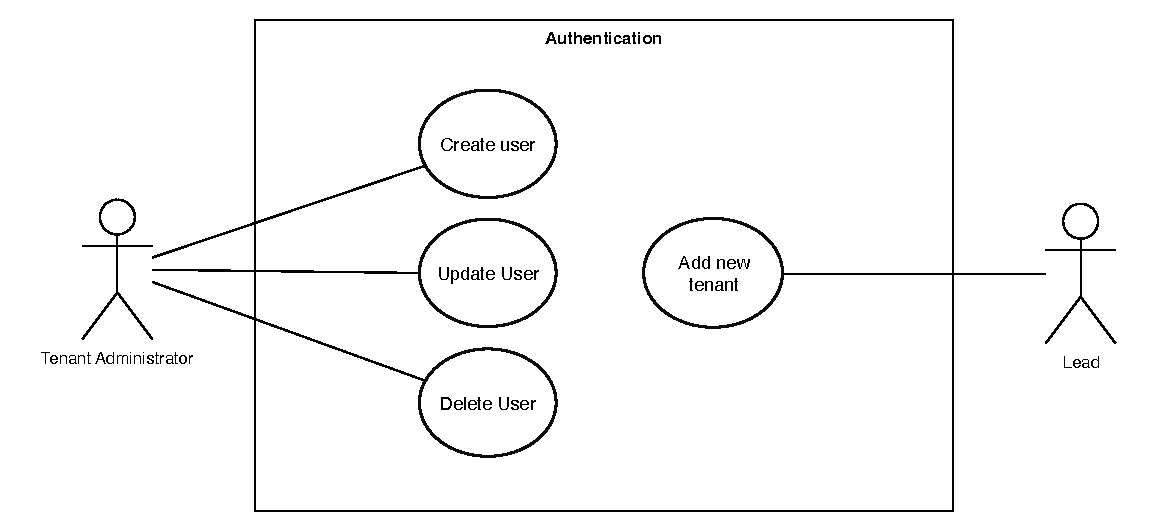
\includegraphics[width=\textwidth]{resources/auth-use-cases.pdf}
    \caption{Authentication Service Use Cases}
    \label{fig:auth-use-cases}
\end{figure}
